\documentclass{article}
\usepackage[utf8]{inputenc}
\usepackage{graphicx}
\usepackage{titling}
\usepackage{titlesec}
\usepackage{booktabs}
\usepackage{fancyhdr}
\usepackage{lipsum}
\usepackage{comment}
\usepackage{enumitem}
\usepackage{listings}
\usepackage{xcolor}
\usepackage{longtable}
\usepackage{cite}
\usepackage{pgfgantt}
\usepackage{amsmath}
\usepackage{tikz}
\usepackage[margin=1in]{geometry}
\usetikzlibrary{calc}


\lstdefinestyle{pidstyle}{
    basicstyle=\ttfamily\footnotesize,
    breaklines=true,
    escapechar=\#, % Define escape character for inline LaTeX commands
    linewidth=\textwidth,
    basicstyle=\ttfamily\scriptsize
}

\renewcommand{\maketitle}{%
  \begin{leftmark}
    \vspace*{\baselineskip} % Add a bit of vertical space

%    \includegraphics[width=4cm]{example-image-a} % Add an image before the title. you will need to replace the image path with your own

%    \vspace{0.5cm} % Add vertical space before title

    \textbf{\fontsize{18}{36}\selectfont \thetitle} % Font Size and Bold Title

     \vspace{0.05cm} % Add vertical space before subtitle
%    \textit{\Large \theauthor}  % Subtitle / Author
    \vspace{\baselineskip} % Add vertical space after subtitle
     \rule{\textwidth}{0.4pt} % Add a horizontal line

   \end{leftmark}
%    \thispagestyle{empty} % Prevent header/footer on the title page
}


% Section Formatting
\titleformat{\section}
  {\normalfont\fontsize{18}{22}\bfseries} % Font and style
  {\thesection}         % Section number
  {1em}                   % Horizontal space after section number
  {}                     % Code before the section name
  []                     % Code after the section name

\titleformat{\subsection}
  {\normalfont\fontsize{14}{18}\bfseries} % Font and style
  {\thesubsection}         % Subsection number
  {1em}                   % Horizontal space after subsection number
  {}                     % Code before the subsection name
  []                     % Code after the subsection name

\setlength{\parindent}{0pt}

\title{Computing platforms (Spring 2025)\newline
week 2}
\author{Juha-Pekka Heikkilä}



\pagestyle{fancy}
\fancyhf{}

\renewcommand{\headrulewidth}{0pt}

\newcommand{\footerline}{\makebox[\textwidth]{\hrulefill}}

\newcommand{\footercontent}{%
    \begin{tabular}{@{}l@{}}
        \footerline \\
        \leftmark \hfill \rlap{\thepage}
    \end{tabular}
}

\fancyfoot[C]{\footercontent}


\newcommand{\exercise}[1]{
    \section*{Exercise #1}
    \markboth{Exercise #1}{}
}



\begin{document}
\maketitle


\exercise{1}
{\bf Multicore. Suppose a single application is running on
a multicore system with 16 processors. If 20\% of the code
is inherently serial, what is the performance gain over
a single processor system? What would it be if only 2\% of
the code would be inherently serial?}
\newline

Using Amdahl's Law \cite{stallings4.3}:
\[
S = \frac{1}{(1 - f) + \frac{f}{N}}
\]
where:
\begin{itemize}
    \item \( 1 - f \): Fraction of the code that is inherently serial.
    \item \( f \): Fraction of the code that is parallelizable.
    \item \( N = 16 \): Number of processors.
\end{itemize}

\begin{enumerate}[label=\textbf{\alph*})]
    \item \textbf{20\% Serial Code (\( 1 - f = 0.2 \), \( f = 0.8 \))}

    Substitute into the formula:
    \[
    S = \frac{1}{(1 - 0.8) + \frac{0.8}{16}} = \frac{1}{0.2 + 0.05} = \frac{1}{0.25} = 4
    \]

    \textbf{Performance Gain:} \( S = 4 \).

    \item \textbf{2\% Serial Code (\( 1 - f = 0.02 \), \( f = 0.98 \))}

    Substitute into the formula:
    \[
    S = \frac{1}{(1 - 0.98) + \frac{0.98}{16}} = \frac{1}{0.02 + 0.06125} = \frac{1}{0.08125} \approx 12.31
    \]

    \textbf{Performance Gain:} \( S \approx 12.31 \).
\end{enumerate}

\newpage

\exercise{2}


We have four jobs that arrive at time 0
\[
\noindent
\begin{aligned}    
A &= 5\text{ ms} \quad \\
B &= 6\text{ ms} \quad \\
C &= 4\text{ ms} \quad \\
D &= 1\text{ ms}
\end{aligned}
\]
All are CPU-bound and we ignore context switch overhead.

\subsection*{(a) Round-Robin with 2 ms time slice}

%\noindent
%\textbf{Timeline Chart:}

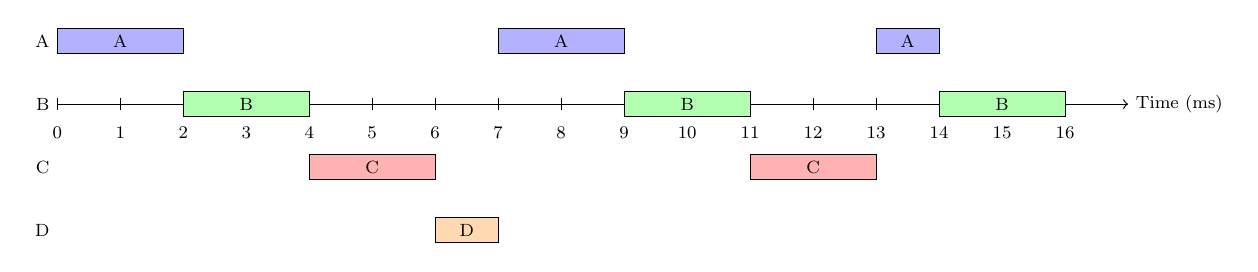
\begin{tikzpicture}[scale=0.8, transform shape, font=\footnotesize]
  % Horizontal axis
  \draw[->] (0,0) -- (17,0) node[right]{Time (ms)};
  % Ticks from 0..16
  \foreach \x in {0,1,2,...,16} {
    \draw (\x,0.1) -- (\x,-0.1) node[below=4pt]{\x};
  }

  \def\drawTime#1#2#3#4#5{
    \draw[fill=#4,draw=black] 
      (#1,#3+0.2) rectangle (#2,#3-0.2) 
      node[midway]{#5};
  }

  % Round-Robin intervals (see bullet list above):

  % (y=1.0)
  \drawTime{0}{2}{1.0}{blue!30}{A}
  \drawTime{7}{9}{1.0}{blue!30}{A}
  \drawTime{13}{14}{1.0}{blue!30}{A}

  % B (y=0.0)
  \drawTime{2}{4}{0.0}{green!30}{B}
  \drawTime{9}{11}{0.0}{green!30}{B}
  \drawTime{14}{16}{0.0}{green!30}{B}

  % C (y=-1.0)
  \drawTime{4}{6}{-1.0}{red!30}{C}
  \drawTime{11}{13}{-1.0}{red!30}{C}

  % D (y=-2.0)
  \drawTime{6}{7}{-2.0}{orange!30}{D}

  % Labels for each job on the left
  \node[left] at (0,1.0) {A};
  \node[left] at (0,0.0) {B};
  \node[left] at (0,-1.0) {C};
  \node[left] at (0,-2.0) {D};
\end{tikzpicture}

\vspace{1em}
\noindent
\textbf{Turnaround times:}
\[
\begin{aligned}
A &\to 14\quad \\
B &\to 16\quad \\
C &\to 13\quad \\
D &\to 7
\end{aligned}
\]

\noindent
\textbf{Average TAT} = \(\frac{14 + 16 + 13 + 7}{4} = 12.5\,\text{ms}\)

\vspace{1em}


\subsection*{(b) First-come-first-served}

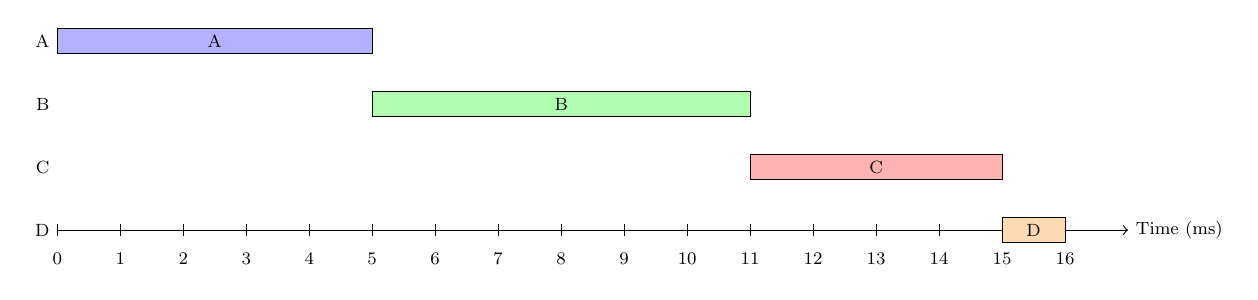
\begin{tikzpicture}[scale=0.8, transform shape, font=\footnotesize]
  \draw[->] (0,0) -- (17,0) node[right]{Time (ms)};
  \foreach \x in {0,1,2,...,16} {
    \draw (\x,0.1) -- (\x,-0.1) node[below=4pt]{\x};
  }

  \def\drawTime#1#2#3#4#5{
    \draw[fill=#4,draw=black] 
      (#1,#3+0.2) rectangle (#2,#3-0.2) 
      node[midway]{#5};
  }

  \drawTime{0}{5}{3.0}{blue!30}{A}
  \drawTime{5}{11}{2.0}{green!30}{B}
  \drawTime{11}{15}{1.0}{red!30}{C}
  \drawTime{15}{16}{0.0}{orange!30}{D}

  \node[left] at (0,3.0) {A};
  \node[left] at (0,2.0) {B};
  \node[left] at (0,1.0) {C};
  \node[left] at (0,0.0) {D};
\end{tikzpicture}

\vspace{1em}
\noindent
\textbf{Turnaround times:}    
\[
    \begin{aligned}
        A &\to 5 \\
        B &\to 11 \\
        C &\to 15 \\
        D &\to 16 \\
    \end{aligned}
\]

\noindent
\textbf{Average TAT} = \(\frac{5 + 11 + 15 + 16}{4} = 11.75\,\text{ms}\)

\newpage

\subsection*{(c) Shortest-job-first}

Order by shortest runtime first: \(D \to C \to A \to B.\) \newline


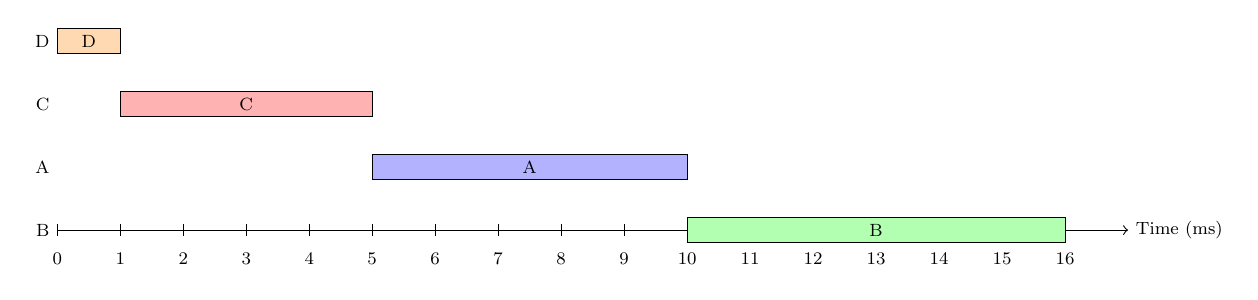
\begin{tikzpicture}[scale=0.8, transform shape, font=\footnotesize]
  \draw[->] (0,0) -- (17,0) node[right]{Time (ms)};
  \foreach \x in {0,1,2,...,16} {
    \draw (\x,0.1) -- (\x,-0.1) node[below=4pt]{\x};
  }

  \def\drawTime#1#2#3#4#5{
    \draw[fill=#4,draw=black] 
      (#1,#3+0.2) rectangle (#2,#3-0.2) 
      node[midway]{#5};
  }

  \drawTime{0}{1}{3.0}{orange!30}{D}
  \drawTime{1}{5}{2.0}{red!30}{C}
  \drawTime{5}{10}{1.0}{blue!30}{A}
  \drawTime{10}{16}{0.0}{green!30}{B}

  \node[left] at (0,3.0) {D};
  \node[left] at (0,2.0) {C};
  \node[left] at (0,1.0) {A};
  \node[left] at (0,0.0) {B};
\end{tikzpicture}

\vspace{1em}
\noindent
\textbf{Turnaround times:}
\[
\begin{aligned}
    D &\to 1 \\
    C &\to 5 \\
    A &\to 10 \\
    B &\to 16 \\
\end{aligned}
\]

\textbf{Average TAT} = \(\frac{1 + 5 + 10 + 16}{4} = 8\,\text{ms}\)

\newpage

\exercise{3}
\begin{enumerate}[label=\textbf{\arabic*}), start=1]
    \item Compute the solutions for simulations with 3 jobs
    and random seeds of 1, 2
    
    
    \begin{enumerate}[label=\textbf{\arabic*}), start=1]
        \item seed 1
        {\scriptsize

        \begin{verbatim}
            $ python3 ./lottery.py -j 3 -s 1
            ARG jlist 
            ARG jobs 3
            ARG maxlen 10
            ARG maxticket 100
            ARG quantum 1
            ARG seed 1
            
            Here is the job list, with the run time of each job: 
            Job 0 ( length = 1, tickets = 84 )
            Job 1 ( length = 7, tickets = 25 )
            Job 2 ( length = 4, tickets = 44 )
            
            
            Here is the set of random numbers you will need (at most):
            Random 651593
            Random 788724
            Random 93859
            Random 28347
            Random 835765
            Random 432767
            Random 762280
            Random 2106
            Random 445387
            Random 721540
            Random 228762
            Random 945271
        \end{verbatim}
        }
    \item seed 2
    {\scriptsize
    \begin{verbatim}
            $ python3 ./lottery.py -j 3 -s 2
            ARG jlist 
            ARG jobs 3
            ARG maxlen 10
            ARG maxticket 100
            ARG quantum 1
            ARG seed 2

            Here is the job list, with the run time of each job: 
            Job 0 ( length = 9, tickets = 94 )
            Job 1 ( length = 8, tickets = 73 )
            Job 2 ( length = 6, tickets = 30 )


            Here is the set of random numbers you will need (at most):
            Random 605944
            Random 606802
            Random 581204
            Random 158383
            Random 430670
            Random 393532
            Random 723012
            Random 994820
            Random 949396
            Random 544177
            Random 444854
            Random 268241
            Random 35924
            Random 27444
            Random 464894
            Random 318465
            Random 380015
            Random 891790
            Random 525753
            Random 560510
            Random 236123
            Random 23858
            Random 325143
    \end{verbatim}
    }

    \end{enumerate}
    \newpage

    \item Now run with two specific jobs: each of length 10,
    but one (job 0) with 1 ticket and the other (job 1) with
    100 (e.g., -l 10:1,10:100). What happens when the number
    of tickets is so imbalanced? Will job 0 ever run before
    job 1 completes? How often? In general, what does such 
    a ticket imbalance do to the behavior of lottery scheduling?

    {\scriptsize
    \begin{verbatim}
        $ python3 ./lottery.py -s 1 -l 10:1,10:100
        ARG jlist 10:1,10:100
        ARG jobs 3
        ARG maxlen 10
        ARG maxticket 100
        ARG quantum 1
        ARG seed 1

        Here is the job list, with the run time of each job: 
        Job 0 ( length = 10, tickets = 1 )
        Job 1 ( length = 10, tickets = 100 )


        Here is the set of random numbers you will need (at most):
        Random 134364
        Random 847434
        Random 763775
        Random 255069
        Random 495435
        Random 449491
        Random 651593
        Random 788724
        Random 93859
        Random 28347
        Random 835765
        Random 432767
        Random 762280
        Random 2106
        Random 445387
        Random 721540
        Random 228762
        Random 945271
        Random 901428
        Random 30590
    \end{verbatim}
    }
    There are total of 101 tickets, 1 for job 0 and 100 for job 1. Job 0
    can run before job 1 finish but it is unlikely. Job 0 has 1/101
    (\(\approx\) 0.99 \%) probability to run before job 1 finish.
    Imbalance causes job 1 'dominate' cpu and job 0 will starve.
\end{enumerate}

\newpage

\exercise{4} Multiprocessor scheduling.
\begin{enumerate}[label=\textbf{\arabic*}), start=1]
    \item The first simulation
    will run just one job, which has a run-time of 30, and a working-set
    size of 200. Run this job (called job ’a’ here) on one simulated CPU
    as follows: ./multi.py -n 1 -L a:30:200. How long will it
    take to complete?
    {\scriptsize
    \begin{verbatim}
        python3 ./multi.py -n 1 -L a:30:200 -c -t
        ARG seed 0
        ARG job_num 3
        ARG max_run 100
        ARG max_wset 200
        ARG job_list a:30:200
        ARG affinity 
        ARG per_cpu_queues False
        ARG num_cpus 1
        ARG quantum 10
        ARG peek_interval 30
        ARG warmup_time 10
        ARG cache_size 100
        ARG random_order False
        ARG trace True
        ARG trace_time False
        ARG trace_cache False
        ARG trace_sched False
        ARG compute True
        
        Job name:a run_time:30 working_set_size:200
        
        Scheduler central queue: ['a']
        
           0   a      
           1   a      
           2   a      
           3   a      
           4   a      
           5   a      
           6   a      
           7   a      
           8   a      
           9   a      
        ----------
          10   a      
          11   a      
          12   a      
          13   a      
          14   a      
          15   a      
          16   a      
          17   a      
          18   a      
          19   a      
        ----------
          20   a      
          21   a      
          22   a      
          23   a      
          24   a      
          25   a      
          26   a      
          27   a      
          28   a      
          29   a      
        
        Finished time 30
        
        Per-CPU stats
        CPU 0  utilization 100.00 [ warm 0.00 ]
    \end{verbatim}
    }
    job will complete in 30 ticks.
    \newpage
    \item  Now increase the cache size so as to make the job’s working
    set (size=200) fit into the cache (which, by default, is size=100);
    for example, run ./multi.py -n 1 -L a:30:200 -M 300. Can you
    predict how fast the job will run once it fits in cache?
    {\scriptsize
    \begin{verbatim}
        $ python3 ./multi.py -n 1 -L a:30:200 -M 300 -c
        ARG seed 0
        ARG job_num 3
        ARG max_run 100
        ARG max_wset 200
        ARG job_list a:30:200
        ARG affinity 
        ARG per_cpu_queues False
        ARG num_cpus 1
        ARG quantum 10
        ARG peek_interval 30
        ARG warmup_time 10
        ARG cache_size 300
        ARG random_order False
        ARG trace False
        ARG trace_time False
        ARG trace_cache False
        ARG trace_sched False
        ARG compute True
        
        Job name:a run_time:30 working_set_size:200
        
        Scheduler central queue: ['a']
        
        
        Finished time 20
        
        Per-CPU stats
          CPU 0  utilization 100.00 [ warm 50.00 ]
    \end{verbatim}
    }
    Now job finish in 20 ticks.
\newpage
    \item Run the same simulation as above, but this time with time
    left tracing enabled (-T). This flag shows both the job that was
    scheduled on a CPU at each time step, as well as how much run-time
    that job has left after each tick has run. What do you notice
    about how that second column decreases?
    {\scriptsize
    \begin{verbatim}
        $ python3 ./multi.py -n 1 -L a:30:200 -M 300 -c -T
        ARG seed 0
        ARG job_num 3
        ARG max_run 100
        ARG max_wset 200
        ARG job_list a:30:200
        ARG affinity 
        ARG per_cpu_queues False
        ARG num_cpus 1
        ARG quantum 10
        ARG peek_interval 30
        ARG warmup_time 10
        ARG cache_size 300
        ARG random_order False
        ARG trace False
        ARG trace_time True
        ARG trace_cache False
        ARG trace_sched False
        ARG compute True
        
        Job name:a run_time:30 working_set_size:200
        
        Scheduler central queue: ['a']
        
           0   a [ 29]      
           1   a [ 28]      
           2   a [ 27]      
           3   a [ 26]      
           4   a [ 25]      
           5   a [ 24]      
           6   a [ 23]      
           7   a [ 22]      
           8   a [ 21]      
           9   a [ 20]      
        ----------------
          10   a [ 18]      
          11   a [ 16]      
          12   a [ 14]      
          13   a [ 12]      
          14   a [ 10]      
          15   a [  8]      
          16   a [  6]      
          17   a [  4]      
          18   a [  2]      
          19   a [  0]      
        
        Finished time 20
        
        Per-CPU stats
          CPU 0  utilization 100.00 [ warm 50.00 ]
    \end{verbatim}
    }
    Once cache warmup is finished, decrease of job time left doubles.
\newpage
    \item Now add one more bit of tracing, to show the status
    of each CPU cache for each job, with the -C flag. For each
    job, each cache will either show a blank space (if the cache
    is cold for that job) or a 'w' (if the cache is warm for that
    job). At what point does the cache become warm for job 'a' in
    this simple example? What happens as you change the warmup time
    parameter (-w) to lower or higher values than the default?

    {\scriptsize
    \begin{verbatim}
        $ python3 ./multi.py -n 1 -L a:30:200 -M 300 -c -T -C
        ARG seed 0
        ARG job_num 3
        ARG max_run 100
        ARG max_wset 200
        ARG job_list a:30:200
        ARG affinity 
        ARG per_cpu_queues False
        ARG num_cpus 1
        ARG quantum 10
        ARG peek_interval 30
        ARG warmup_time 10
        ARG cache_size 300
        ARG random_order False
        ARG trace False
        ARG trace_time True
        ARG trace_cache True
        ARG trace_sched False
        ARG compute True
        
        Job name:a run_time:30 working_set_size:200
        
        Scheduler central queue: ['a']
        
           0   a [ 29] cache[ ]     
           1   a [ 28] cache[ ]     
           2   a [ 27] cache[ ]     
           3   a [ 26] cache[ ]     
           4   a [ 25] cache[ ]     
           5   a [ 24] cache[ ]     
           6   a [ 23] cache[ ]     
           7   a [ 22] cache[ ]     
           8   a [ 21] cache[ ]     
           9   a [ 20] cache[w]     
        -------------------------
          10   a [ 18] cache[w]     
          11   a [ 16] cache[w]     
          12   a [ 14] cache[w]     
          13   a [ 12] cache[w]     
          14   a [ 10] cache[w]     
          15   a [  8] cache[w]     
          16   a [  6] cache[w]     
          17   a [  4] cache[w]     
          18   a [  2] cache[w]     
          19   a [  0] cache[w]     
        
        Finished time 20
        
        Per-CPU stats
          CPU 0  utilization 100.00 [ warm 50.00 ]
    \end{verbatim}
    }
    When cache warmup has happened ticks remaining for job start to
    decrease faster, shorter warmup time will reduce total ticks faster
    making total time for job shorter.
\end{enumerate}
\newpage

\exercise{5} 
Multiprocessor scheduling (cont’d). We continue from previous exercise,
that is, use the simulator multi.py as in previous exercise, and
answer the homework questions 5-7 from OSTEP Chapter 10.

\begin{enumerate}[label=\textbf{\arabic*}), start=5]
    \item Let's run the following three jobs on a two-CPU system
    (i.e., type ./multi.py -n 2 -L a:100:100,b:100:50,c:100:50)
    Can you predict how long this will take, given a round-robin
    centralized scheduler? Use -c to see if you were right, and
    then dive down into details with -t.
    {\scriptsize
    \begin{verbatim}
        $ python3 ./multi.py -n 2 -L a:100:100,b:100:50,c:100:50 -c
        ARG seed 0
        ARG job_num 3
        ARG max_run 100
        ARG max_wset 200
        ARG job_list a:100:100,b:100:50,c:100:50
        ARG affinity 
        ARG per_cpu_queues False
        ARG num_cpus 2
        ARG quantum 10
        ARG peek_interval 30
        ARG warmup_time 10
        ARG cache_size 100
        ARG random_order False
        ARG trace False
        ARG trace_time False
        ARG trace_cache False
        ARG trace_sched False
        ARG compute True
        
        Job name:a run_time:100 working_set_size:100
        Job name:b run_time:100 working_set_size:50
        Job name:c run_time:100 working_set_size:50
        
        Scheduler central queue: ['a', 'b', 'c']
        
        
        Finished time 150
        
        Per-CPU stats
          CPU 0  utilization 100.00 [ warm 0.00 ]
          CPU 1  utilization 100.00 [ warm 0.00 ]
    \end{verbatim}
    }
    Jobs finish with 150 ticks. Dummy round robin scheduling without
    considering job cpu history cause losing caches often.

\newpage
    \item Now we’ll apply some explicit controls to study
    cache affinity, as described in the chapter. To do this,
    you'll need the -A flag. This flag can be used to limit which
    CPUs the scheduler can place a particular job upon.
    Can you predict how fast this version will run? Why does it
    do better? Will other combinations of 'a', 'b', and 'c' onto
    the two processors run faster or slower?
    {\scriptsize
    \begin{verbatim}
        $ python3 ./multi.py -n 2 -L a:100:100,b:100:50,c:100:50 -A a:0,b:1,c:1 -c
        ARG seed 0
        ARG job_num 3
        ARG max_run 100
        ARG max_wset 200
        ARG job_list a:100:100,b:100:50,c:100:50
        ARG affinity a:0,b:1,c:1
        ARG per_cpu_queues False
        ARG num_cpus 2
        ARG quantum 10
        ARG peek_interval 30
        ARG warmup_time 10
        ARG cache_size 100
        ARG random_order False
        ARG trace False
        ARG trace_time False
        ARG trace_cache False
        ARG trace_sched False
        ARG compute True
        
        Job name:a run_time:100 working_set_size:100
        Job name:b run_time:100 working_set_size:50
        Job name:c run_time:100 working_set_size:50
        
        Scheduler central queue: ['a', 'b', 'c']
        
        
        Finished time 110
        
        Per-CPU stats
          CPU 0  utilization 50.00 [ warm 40.91 ]
          CPU 1  utilization 100.00 [ warm 81.82 ]
    \end{verbatim}
    }
    Jobs finish now at 110 (instead of 150) because caches are not
    lost.
\newpage
    \item One interesting aspect of caching multiprocessors is
    the opportunity for better-than-expected speed up of jobs
    when using multiple CPUs (and their caches) as compared to
    running jobs on a single processor. Specifically, when you
    run on N CPUs, sometimes you can speed up by more than
    a factor of N, a situation entitled super-linear speedup.
    What do you notice about performance as the number of CPUs
    scales? Use -c to confirm your guesses, and other tracing
    flags to dive even deeper.
    {\scriptsize
    \begin{verbatim}
        $ python3 ./multi.py -n 3 -L a:100:100,b:100:100,c:100:100 -M 100  -c
        ARG seed 0
        ARG job_num 3
        ARG max_run 100
        ARG max_wset 200
        ARG job_list a:100:100,b:100:100,c:100:100
        ARG affinity 
        ARG per_cpu_queues False
        ARG num_cpus 3
        ARG quantum 10
        ARG peek_interval 30
        ARG warmup_time 10
        ARG cache_size 100
        ARG random_order False
        ARG trace False
        ARG trace_time False
        ARG trace_cache False
        ARG trace_sched False
        ARG compute True
        
        Job name:a run_time:100 working_set_size:100
        Job name:b run_time:100 working_set_size:100
        Job name:c run_time:100 working_set_size:100
        
        Scheduler central queue: ['a', 'b', 'c']
        
        
        Finished time 55
        
        Per-CPU stats
          CPU 0  utilization 100.00 [ warm 81.82 ]
          CPU 1  utilization 100.00 [ warm 81.82 ]
          CPU 2  utilization 100.00 [ warm 81.82 ]
    \end{verbatim}
    }
    When CPU \# equal to job \# and cache size is big enough to fit
    working set caches are never lost hence caches after warmup
    operate optimally.
\end{enumerate}

\newpage
\bibliographystyle{plain}
\bibliography{references}
\end{document}